\documentclass[brazil,pagestart=firstchapter]{abnt}

% This does not accept all Unicode chars (for instance: I²C gives an error)
%\usepackage[utf8]{inputenc}

% This adds support for Unicode chars.
\usepackage{ucs}
\usepackage[utf8x]{inputenc}
% But should be avoided:
% http://tex.stackexchange.com/questions/13067/utf8x-vs-utf8-inputenc

\usepackage[brazil]{babel}

% http://tex.stackexchange.com/questions/664/why-should-i-use-usepackaget1fontenc
% http://texblog.net/latex-archive/fonts/symbols/
\usepackage[T1]{fontenc}

% Use another font:
% http://tex.stackexchange.com/questions/553/what-packages-do-people-load-by-default-in-latex/951#951
%\usepackage{lmodern}

% 'microtype' improves LaTeX line-breaking algorithm by using
% microtypographic features of the font
% http://tex.stackexchange.com/questions/349/what-is-the-practical-difference-between-latex-and-pdflatex/358#358
\usepackage{microtype}


%%%%%%%%%%%%%%%%%%%%%%%%%%%%%%%%%%%%%%%%%%%%%%%%%%%%%%%%%%%%
% Acronyms and abbreviations

% Simple and effective acronym package:
\usepackage[printonlyused,withpage]{acronym}

% This one from abntex does not work correctly:
% http://comments.gmane.org/gmane.comp.tex.brazilian/13365
%\usepackage{tabela-simbolos}

% "nomencl" is quite annoying to use, specially when compared to "acronym".
% "nomencl" requires an external file and some extra commands.
% "acronym", on the other hand, just works out of the box!
%\usepackage{nomencl}
%\makenomenclature
% http://en.wikibooks.org/wiki/LaTeX/Indexing#Abbreviation_list
% http://franz.kollmann.in/latex/latex.html#abbr
% latexmk needs a custom dependency for this package
% http://magic.aladdin.cs.cmu.edu/2007/11/06/continuous-latex-compilation-using-latexmk/


%%%%%%%%%%%%%%%%%%%%%%%%%%%%%%%%%%%%%%%%%%%%%%%%%%%%%%%%%%%%
% Other packages

% Adding \textsubscript{}
% LaTeX already has \textsuperscript, but lacks \textsubscript.
% http://en.wikibooks.org/wiki/LaTeX/Formatting#Text_mode_superscript_and_subscript
\usepackage{fixltx2e}

% Better handling of space after a custom command.
% http://tex.stackexchange.com/questions/17730/newcommand-and-spacing
\usepackage{xspace}

% Avoid floats and figures from crossing a section boundary
% http://en.wikibooks.org/wiki/LaTeX/Floats,_Figures_and_Captions#Keeping_floats_in_their_place
\usepackage[section]{placeins}

% Required for including graphics
\usepackage{graphicx}

% Inserting PDF pages from other documents
%\usepackage{pdfpages}
% TODO: remove "draft" here!
\usepackage[draft]{pdfpages}

% SI Units
% https://bitbucket.org/josephwright/siunitx/issue/100/undefined-control-sequence-bit-and-byte
\usepackage{siunitx}
\sisetup{
	load-configurations = binary,
	per-mode = symbol,
	list-final-separator = { e },
	range-phrase = { a },
	output-decimal-marker = {,}
}
\DeclareSIUnit\gauss{G}

% To find the total number of pages
%\usepackage{lastpage}

%%%%%%%%%%%%%%%%%%%%%%%%%%%%%%%%%%%%%%%%%%%%%%%%%%%%%%%%%%%%
% Embedding source-code

%\usepackage{color}
%\usepackage{xcolor}

% LaTeX, as delivered, offers no means of handling bold "teletype" fonts
% http://www.tex.ac.uk/cgi-bin/texfaq2html?label=bold-extras
% http://tex.stackexchange.com/questions/33039/using-ttfamily-with-bfseries-or-how-to-enable-bold-in-fixed-width-font
% And the solution is to load another fixed-width font:
%\usepackage{courier}
%\usepackage{couriers}
%\usepackage{beramono}
% Either load all fonts from this pack:
\usepackage{txfonts}
% Or load only the typewriter one.
%\renewcommand{\ttdefault}{txtt}

% For inserting source-code
\usepackage{listings}

% Setting the default options
\lstset{
	basicstyle=\ttfamily\footnotesize,
	numberstyle=\scriptsize,
	numbers=left,
	escapeinside={(*@}{@*)},
	tabsize=4,
	breaklines=true,
	breakatwhitespace=true,
	showspaces=false,
	showstringspaces=false,
	showlines=false
}
%	extendedchars=true,
%	inputencoding=utf8x,
%	numbersep=5pt,
%	frame=shadowbox,
%	frameround=rrrt,
%	rulecolor=\color{black},
%	rulesepcolor=\color{black},


% AVISO!!!  (copiado de outro projeto, mas não se aplica aqui)
% Dentro dos exemplos de código-fonte abaixo, coloquei um "tab" de
% indentação por estar dentro de um "frame", e "espaços" para a
% indentação do código de exemplo. Isto foi necessário porque os tabs
% estavam sendo ignorados dentro do códigos de exemplo.

\lstnewenvironment{ccode}[1][]
{\lstset{language=C,
	#1}
}{}

\lstnewenvironment{pythoncode}[1][]
{\lstset{language=Python,
	#1}
}{}

\lstnewenvironment{shellcode}[1][]
{\lstset{language=bash,
	#1}
}{}

% \begin{lstlisting}[caption={Useless code},label=useless]
% \end{lstlisting}


%%%%%%%%%%%%%%%%%%%%%%%%%%%%%%%%%%%%%%%%%%%%%%%%%%%%%%%%%%%%
% Table-related packages:

% For multirow cells inside tabular environments
%\usepackage{multirow}

% Longtable allows you to write tables that continue to the next page
%\usepackage{longtable}

% 'tabularx' package - simple column stretching
% http://en.wikibooks.org/wiki/LaTeX/Tables#The_tabularx_package_-_simple_column_stretching
%\usepackage{tabularx}

% 'booktabs' - Publication quality tables in LaTeX
%\usepackage{booktabs}

% Alternating row colors in tables
%\usepackage[table]{xcolor}
%\definecolor{tabular-odd-color}{gray}{0.90}
%\definecolor{tabular-even-color}{gray}{0.97}


%%%%%%%%%%%%%%%%%%%%%%%%%%%%%%%%%%%%%%%%%%%%%%%%%%%%%%%%%%%%
% Fancy headers (and footers)
% http://en.wikibooks.org/wiki/LaTeX/Page_Layout#Page_Styles
%\usepackage{fancyhdr}
%\pagestyle{fancy}
%
%% Headers and footers definition:
%\lhead{\includegraphics[height=21mm]{shared/2aliancas_h.pdf}}
%\chead{}
%% This \parbox is a hack to keep text aligned at top, but it's not the
%% only available solution:
%% http://tex.stackexchange.com/questions/2440/how-to-vertically-align-headers-footers-in-fancyhdr-package
%\rhead{\parbox[b][21mm][t]{0.65\textwidth}{\raggedleft\large\titletext \\[1em] \subtitletext}}
%\lfoot{}
%\cfoot{}
%\rfoot{Page \thepage{} of \pageref{LastPage}}
%
%\renewcommand{\headrulewidth}{0pt}  % Default is 0.4pt
%\renewcommand{\footrulewidth}{0pt}  % Default is 0pt


%%%%%%%%%%%%%%%%%%%%%%%%%%%%%%%%%%%%%%%%%%%%%%%%%%%%%%%%%%%%
% 'hyperref' for including hyperlinks to the PDF.
% It should be loaded last.
% http://en.wikibooks.org/wiki/LaTeX/Formatting#Typesetting_URLs
\usepackage{hyperref}
\hypersetup{
	pdfborder={0 0 0},
	hyperindex=false
}
% hyperindex=false is required by "tabela-de-simbolos"

% http://en.wikibooks.org/wiki/LaTeX/Labels_and_Cross-referencing#Issues_with_links_to_tables_and_figures_handled_by_hyperref
%\usepackage[all]{hypcap}


%%%%%%%%%%%%%%%%%%%%%%%%%%%%%%%%%%%%%%%%%%%%%%%%%%%%%%%%%%%%
% Custom commands
% http://tex.stackexchange.com/questions/1050/whats-the-difference-between-newcommand-and-newcommand

% http://tex.stackexchange.com/questions/24132/overline-outside-of-math-mode
\makeatletter
\newcommand*{\textoverline}[1]{$\overline{\hbox{#1}}\m@th$}
\makeatother

% http://tex.stackexchange.com/questions/15009/macros-for-common-abbreviations
\newcommand*{\eg}{e.g.\@\xspace}
\newcommand*{\ie}{i.e.\@\xspace}

\newcommand*{\VBUS}{V\textsubscript{BUS}\xspace}
\newcommand*{\VCC}{V\textsubscript{CC}\xspace}
\newcommand*{\VDD}{V\textsubscript{DD}\xspace}
\newcommand*{\GND}{GND\xspace}
% http://tex.stackexchange.com/questions/9691/avoid-hyphenation-in-2-d
\newcommand*{\VUSB}{\mbox{V-USB}\xspace}

%%%%%%%%%%%%%%%%%%%%%%%%%%%%%%%%%%%%%%%%%%%%%%%%%%%%%%%%%%%%
% Other notes

% \linewidth is either \columnwidth in two-column mode or \textwidth in one-column mode.
% http://tex.stackexchange.com/questions/275/how-to-find-the-textwidth-in-two-column-mode/3531#3531

%%%%%%%%%%%%%%%%%%%%%%%%%%%%%%%%%%%%%%%%%%%%%%%%%%%%%%%%%%%%
% Some metadata

% This is used only by latex-beamer package:
%\title{Mouse USB usando magnetômetro}
%\author{Denilson Figueiredo de Sá}
%\date{2011-11-16}
%\institute{DCC/UFRJ}
%\keywords{AVR, USB, mouse, magnetometer}

\autor{Denilson Figueiredo de Sá}
\titulo{Mouse USB usando magnetômetro}
\orientador{Nelson Quilula Vasconcelos}
%\comentario{}
\instituicao{Departamento de Ciência da Computação \par Instituto de Matemática \par Universidade Federal do Rio de Janeiro}
\local{Rio de Janeiro - RJ, Brasil}
\data{16 de novembro de 2011}

% latex-beamer sets the pdftitle and pdfauthor automatically, but here we
% must explicitly run it:
\hypersetup{
	pdftitle={\ABNTtitulodata},
	pdfauthor={\ABNTautordata}
}

%%%%%%%%%%%%%%%%%%%%%%%%%%%%%%%%%%%%%%%%%%%%%%%%%%%%%%%%%%%%
\begin{document}

% The "abnt" class issues a warning:
%   pdfTeX warning (ext4): destination with the same identifier
%   (name{page.i}) has been already used, duplicate ignored
% This page has a solution (or workaround):
% http://en.wikibooks.org/wiki/LaTeX/Hyperlinks#Problems_with_Links_and_Pages
%\pagenumbering{roman}
% But, anyway, it's better to ignore that warning (or even better would be
% to report it to abntex maintainers).
% Instead of messing with page numbering, I've added pagestart=firstchapter
% option.


\capa

\folhaderosto


\begin{folhadeaprovacao}

\setlength{\ABNTsignthickness}{0.4pt}
\setlength{\ABNTsignskip}{2cm}
\hspace*{1cm}

\centerline{\textbf{\large \ABNTtitulodata}}

\bigskip
\bigskip

\centerline{\textbf{\ABNTautordata}}

\bigskip
\bigskip

Projeto Final de Curso submetido ao Departamento de Ciência da Computação
do Instituto de Matemática da Universidade Federal do Rio de Janeiro como
parte dos requisitos necessários para obtenção do grau de Bacharel em
Ciência da Computação.

Apresentado por:

\assinatura{\ABNTautordata}

Aprovado por:

\assinatura{Prof. Nelson Quilula Vasconcelos \\ Orientador}
\assinatura{Prof. Adriano Joaquim}
\assinatura{Profª. Silvana Rossetto}

\bigskip
\bigskip
\bigskip

\begin{center}
\ABNTlocaldata

\ABNTdatadata
\end{center}

\end{folhadeaprovacao}


% Colocar o Sumário aqui é muito bom, mas não é de acordo com a norma ABNT
% NBR 14724: informação e documentação: trabalhos acadêmicos: apresentação.
%\tableofcontents{}


%\pretextualchapter{Dedicatória}
% TODO: escrever dedicatória (opcional)

%\pretextualchapter{Agradecimentos}
% TODO: escrever agradecimentos


\begin{resumo}
O resumo será escrito aqui.
\end{resumo}

\begin{abstract}
This will be the abstract, someday.
\end{abstract}


\listoffigures

%\listoftables


% The following command does not work:
% \listadesiglas
% Instead, I'm using "acronym" package.

\pretextualchapter{Lista de Siglas}

\begin{acronym}[EEPROM]

\acro{USB}{Universal Serial Bus}
\acro{HID}{Human Interface Device}

\acro{NRZI}{Non-Return-to-Zero Inverted}
\acro{SE0}{Single-Ended 0}
\acro{SE1}{Single-Ended 1}

\acro{I2C}[I²C]{Inter-Integrated Circuit}
\acro{TWI}{Two-Wire Interface}

\acro{SCL}{Serial Clock}
\acro{SDA}{Serial Data}

\acro{PDIP}{Plastic Dual In-line Package}
\acro{DIP}{Dual In-line Package}
\acro{QFP}{Quad Flat Package}
\acro{QFN}{Quad-Flat No-leads Package}
\acro{LCC}{Leaded Chip Carrier}

\acro{PCB}{Printed Circuit Board}
\acro{LED}{Light-Emitting Diode}
\acro{ADC}{Analog-to-Digital Converter}

\acro{ISP}{In-System Programmer}
\acro{ICSP}{In-Circuit Serial Programmer}

\acro{SRAM}{Static Random-Access Memory}
\acro{ROM}{Read-Only Memory}
\acro{EEPROM}{Electrically Erasable Programmable Read-Only Memory}

\acro{API}{Application Programming Interface}

\end{acronym}


\tableofcontents


\chapter{Introdução}
\label{cap:introducao}

Falar sobre: motivação, resumo, possíveis aplicações (palestras,
necessidades especiais, interatividade em jogos e exposições)

\section{Trabalhos relacionados}
\label{sec:trabalhos_relacionados}

\subsection{TrackIR}
\label{sub:trackir}

% http://www.naturalpoint.com/trackir/

\subsection{Wiimote}
\label{sub:wiimote}

% http://en.wikipedia.org/wiki/Wiimote
% http://wiibrew.org/wiki/Wiimote

\subsection{Eye-tracking}
\label{sub:eyetracking}

% http://www.technologyreview.com/Infotech/18254/
% http://hci.stanford.edu/research/GUIDe/applications.html
% http://www.bltt.org/pointer/index.htm#gen9
% http://www.inference.phy.cam.ac.uk/dasher/SpecialNeeds.html
% http://www.inference.phy.cam.ac.uk/dasher/Headmouse.html


\chapter{Protocolos e componentes}
\label{cap:protocolos_e_componentes}

\section{USB}
\label{sec:usb}

\ac{USB} é um protocolo que foi desenvolvido a partir do ano de 1994 pelas
empresas \textit{Compaq}, \textit{Hewlett-Packard}, \textit{Intel},
\textit{Lucent}, \textit{Microsoft}, \textit{NEC} e \textit{Philips}. Foi
motivado pela inexistência de um barramento bidirecional de baixo custo para
periféricos de baixa e média velocidade, assim como a falta de flexibilidade
dos barramentos até então existentes, os quais eram projetados para usos
bastante específicos, sendo impossível reutilizá-los para outros
periféricos. \cite{usb20}

A primeira versão do \ac{USB}, conhecida como ``USB 1.0'', foi oficialmente
lançada em janeiro de 1996 e definiu duas velocidades: \textit{low speed}
(\SI{1.5}{\mega\bit\per\second}) e \textit{full speed}
(\SI{12}{\mega\bit\per\second}). Alguns anos depois, em setembro de 1998, foi
lançada sua primeira revisão, ``USB 1.1'', que resolveu alguns problemas da
versão anterior mas não introduziu nenhuma mudança significativa.

A primeira grande revisão do protocolo foi lançada em abril de 2000, com o
nome de ``USB 2.0''. Esta versão introduziu uma terceira velocidade --
\textit{high speed} (\SI{480}{\mega\bit\per\second}) -- mas manteve total
compatibilidade com a revisão anterior do protocolo: dispositivos USB 1.x
funcionam em \textit{hosts} USB 2.0, e dispositivos USB 2.0 funcionam em
\textit{hosts} USB 1.x (porém limitados a \textit{full speed}).

\begin{figure}[h]
\centering
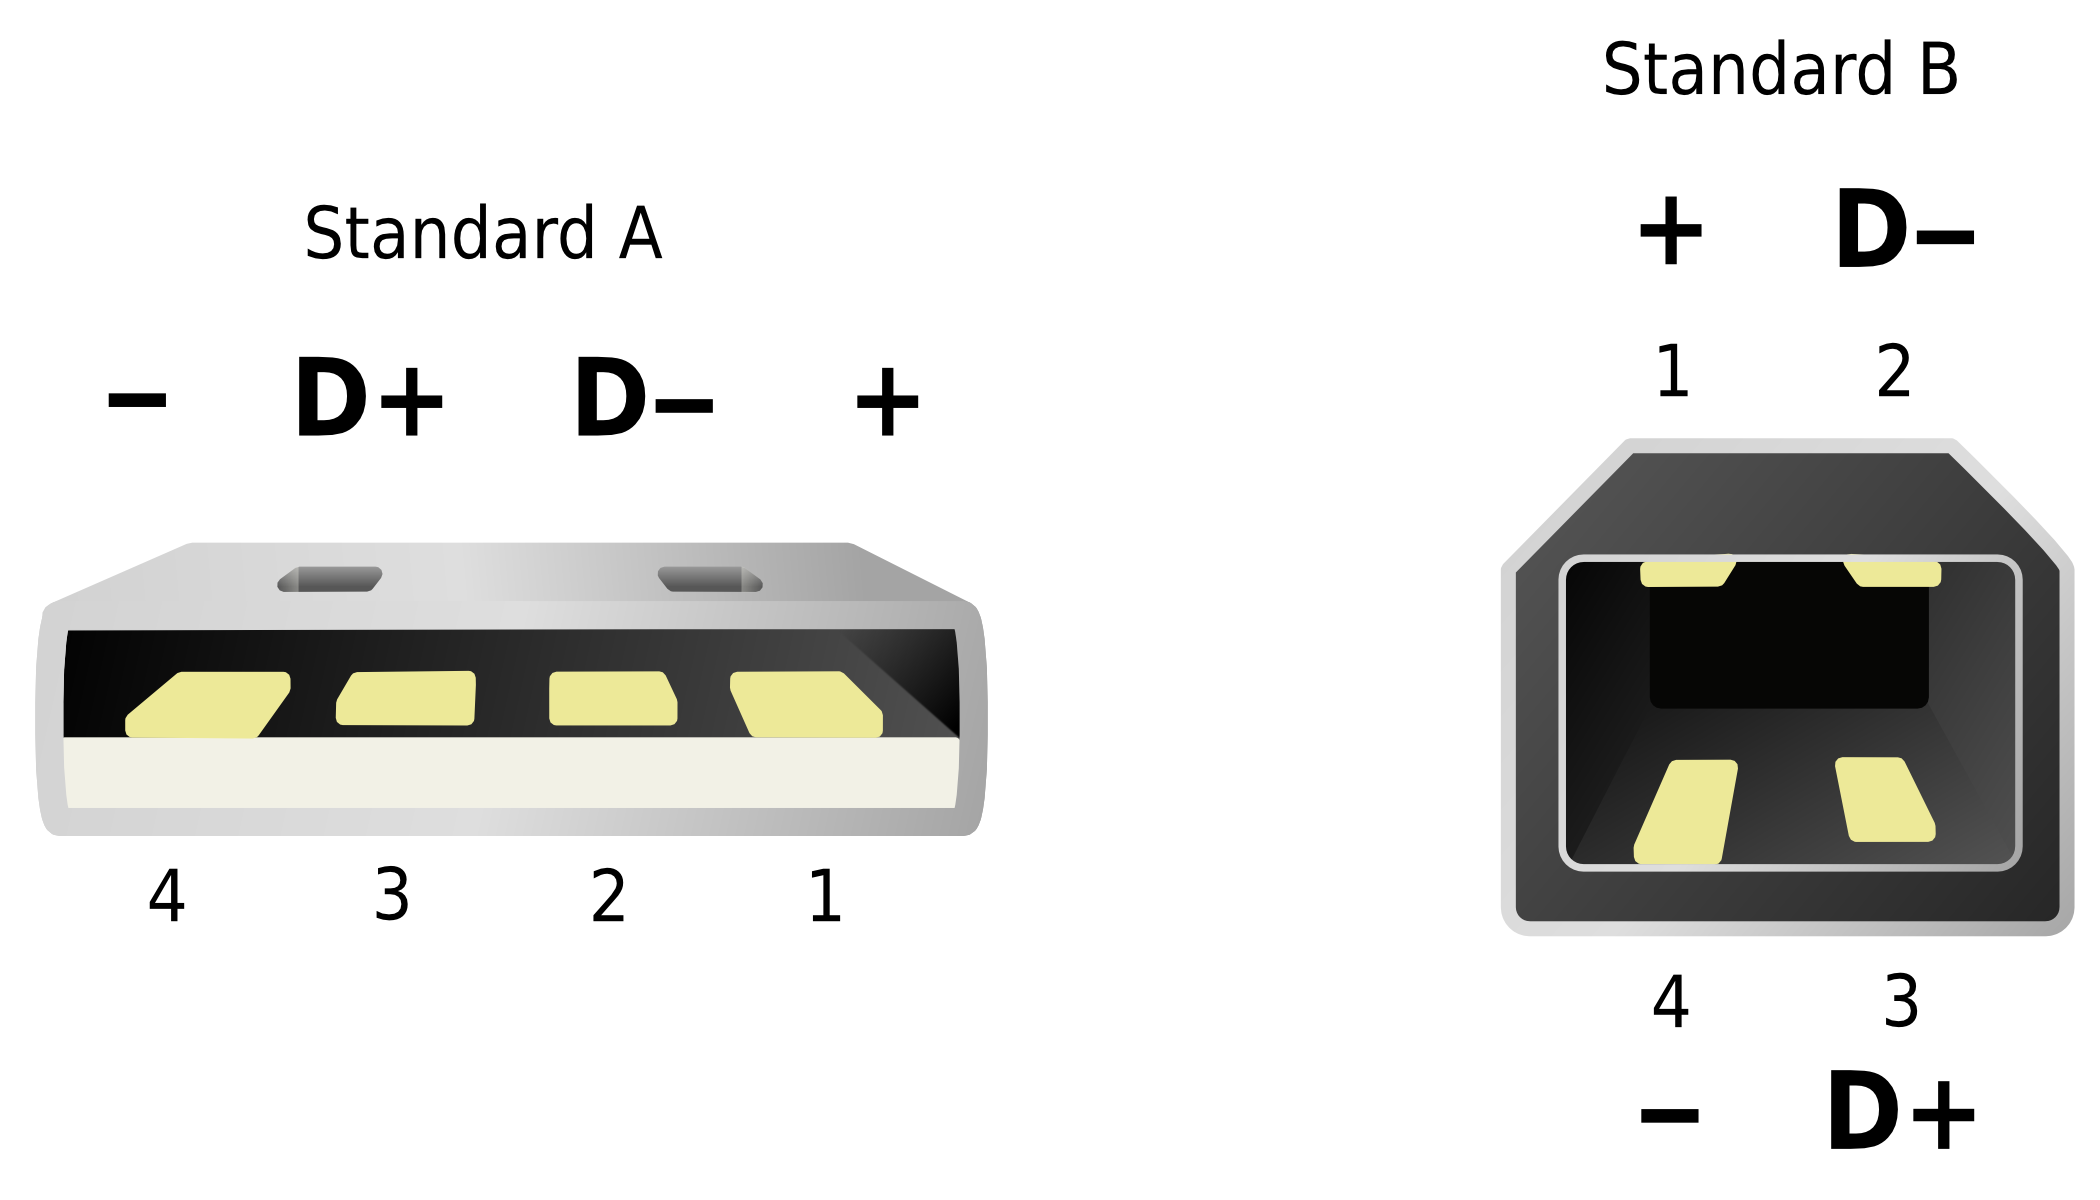
\includegraphics[width=0.5\textwidth]{img/USB.png}
\caption{Conectores do tipo A e do tipo B para USB 1.x/2.0}
\label{fig:usb_connectors}
\end{figure}

Uma conexão \ac{USB} é formada por 4 vias, sendo duas para alimentação
(\VBUS = \SI{+5}{\volt} e \GND) e duas para comunicação (D+ e D-). Os dados
são transmitidos usando a codificação \ac{NRZI} com \textit{bit stuffing}
(um ``zero'' é inserido após 6 bits ``um'' consecutivos).
\cite[p.~157]{usb20} \cite[cap.~2]{usbinanutshell}

A velocidade de um dispositivo é determinada por \textit{hardware}, de
acordo com a posição do resistor de \textit{pull-up}\footnote{
	Resistores de \textit{pull-up} ou de \textit{pull-down} servem para
	manter uma via de dados num nível lógico conhecido enquanto nenhuma
	transferência ocorre.  Normalmente possuem um valor relativamente alto
	(de \SIrange{1.5}{15}{\kilo\ohm}) para drenar pouca corrente. Um
	resistor de \textit{pull-up} conecta a via ao \VDD e a mantém no nível
	lógico 1, enquanto um resistor de \textit{pull-down} conecta a via ao
	\GND e a mantém no nível lógico 0.}
nas vias de dados. Dispositivos
\textit{low speed} possuem um resistor de \textit{pull-up} ligado ao D-,
enquanto dispositivos \textit{full speed} possuem  um resistor de
\textit{pull-up} ligado ao D+. Se não há nenhum resistor de
\textit{pull-up}, assume-se que não há nenhum dispositivo conectado.
\cite[p.~141]{usb20} \cite[cap.~2]{usbinanutshell}

Dispositivos \textit{high speed}, introduzidos no \ac{USB} 2.0, inicialmente
se identificam como \textit{full speed} (com um resistor de \textit{pull-up}
ligado ao D+), mas removem o resistor após uma negociação realizada durante
o durante o USB \textit{reset}, caso o \textit{host} também suporte
\textit{high speed}.  Caso contrário, o resistor será mantido e o
dispositivo funcionará em \textit{full speed}. Essa negociação incial
permite a compatibilidade entre dispositivos USB 2.0 \textit{high speed} e
\textit{hosts} USB 1.x. \cite[p.~142]{usb20} \cite[cap.~2]{usbinanutshell}

\begin{figure}[h]
\centering
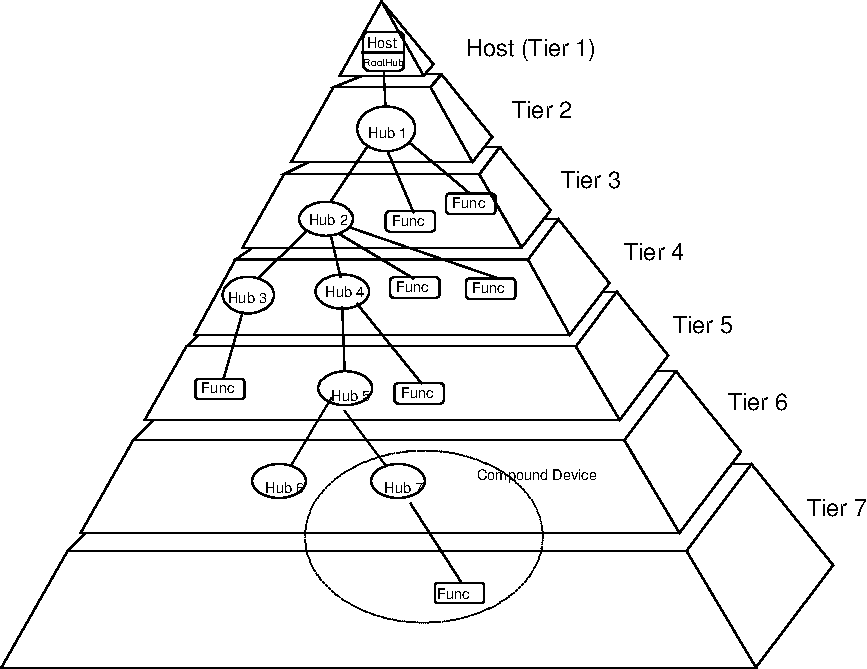
\includegraphics[width=0.75\textwidth]{img/usb_bus_topology.pdf}
\caption{Topologia do barramento USB}
\label{fig:usb_topology}
\end{figure}

A conexão de equipamentos \ac{USB} segue uma topologia de estrela em
camadas, que também pode ser entendida como uma árvore. No centro da estrela
(ou na raiz da árvore) temos obrigatoriamente o \textit{host}, que
normalmente é um computador. Por definição, o \textit{host} contém um
\textit{root hub}. Cada cabo \ac{USB} é uma conexão ponto-a-ponto que liga
um \textit{hub} da camada imediatamente acima a um dispositivo na camada
imediatamente abaixo. Um dispositivo pode ser um outro \textit{hub} ou então
uma função. Por limitações de tempo de propagação, o número máximo de
camadas é 7, incluindo a camada que contém o \textit{host}.
\cite[p.~16]{usb20}

A especificação \ac{USB} define dois tipos de conectores (conforme ilustrado
na figura \ref{fig:usb_connectors}). Um cabo \ac{USB} possui uma ponta de
cada tipo, sendo que o plugue do tipo A é conectado ao \textit{hub} da
camada acima, e o plugue do tipo B é conectado ao dispositivo da camada
abaixo. Posteriormente, foram também especificados conectores de tamanho
mais reduzido (Mini e Micro), mas os conceitos continuam os mesmos.

O protocolo de comunicação do \ac{USB} pode ser entendido como uma
arquitetura \textit{master/slave}, na qual o \textit{host} é o
\textit{master} e os dispositivos têm o papel de \textit{slave}. Só há um
\textit{host} por barramento \ac{USB}, e ele é responsável por iniciar e
gerenciar cada transação.  Como consequência, a maior parte da lógica está
centralizada no \textit{host}, simplificando bastante a implementação de
dispositivos que se conectam ao barramento \ac{USB}. \cite{usbinanutshell}

Em novembro de 2008, foi lançada a especificação do USB 3.0, que introduziu
uma quarta velocidade: \textit{super speed} (\SI{5}{\giga\bit\per\second}).
A quantidade de mudanças para suportar essa nova velocidade é grande, e foge
ao escopo deste trabalho.

% Não falei sobre:
% * Descriptors
% * * Device Descriptor
% * * Configuration Descriptor
% * * Interface Descriptor
% * * Endpoint Descriptor
% * * String Descriptor

\subsection{\textit{Endpoints}}
\label{sub:usb_endpoints}

Um \textit{endpoint} pode ser visto como um endereço lógico que pode receber
dados do \textit{host} ou enviar dados para ele. Todo dispositivo \ac{USB}
possui o \textit{endpoint 0}, usado pelo próprio protocolo para mensagens de
controle e de \textit{status}. \cite[cap.~3]{usbinanutshell}

Além do \textit{endpoint 0}, um dispositivo \ac{USB} normalmente possui no
mínimo mais 1 \textit{endpoint}, usado para o objetivo fim do dispositivo.

Há 4 tipos de \textit{endpoints}: \cite[cap.~4]{usbinanutshell}

TODO FROM HERE

% * Endpoints e tipos de transferências
% * *(control, interrupt, isochronous, bulk)


\section{USB HID}
\label{sec:usb_hid}

De modo a permitir a existência de dispositivos \textit{plug-and-play} --
que funcionam assim que são ligados ao \textit{host}, sem necessidade de
configurações feitas pelo usuário ou de instalação de drivers específicos --
foram definidas algumas classes de dispositivos. Por exemplo, os populares
\textit{pen drives}, que substituíram os disquetes e CDs regraváveis para
transferência de arquivos, pertencem à classe \textit{USB Mass Storage}, e
os sistemas operacionais modernos já incluem suporte nativo a dispositivos
dessa classe.

Dispositivos de interface com seres humanos fazem parte da classe
\textit{USB \ac{HID}} e abrangem principalmente teclados, mouses e
joysticks. No entanto, essa classe foi projetada de forma genérica, e inclui
outros tipos de dispositivos com necessidades similares, tais como medidores
de temperatura, controles de um painel (botões, alavancas, ajustes),
volantes, pedais, leitores de códigos de barra, ou ainda novos dispositivos
que não foram previstos inicialmente na especificação. \cite[p.~1]{usbhid}

A classe \ac{USB} \ac{HID} tem como objetivos ser compacta (para reduzir o
espaço necessário no \textit{firmware} do dispositivo), ser flexível e
extensível, ser genérica e auto-descritiva (de modo que cada dispositivo
descreva suas características de forma padronizada para o \textit{host}). O
driver da classe \ac{USB} \ac{HID}, presente no sistema operacional, é capaz
de se comunicar com qualquer dispositivo dessa classe. \cite[p.~2]{usbhid}

A especificação do \ac{USB} \ac{HID} foi inicialmente lançada em janeiro de
1996 (versão 1.0). Sua primeira revisão ficou disponível em abril de 1999
(versão 1.1). Sua segunda revisão, que também é a mais recente, foi lançada
em junho de 2001 (versão 1.11). Apesar desta versão ter sido lançada após o
\ac{USB} 2.0, a especificação do \ac{USB} \ac{HID} menciona apenas as duas
velocidades de dispositivos presentes no \ac{USB} 1.x, e incorretamente
chama dispositivos \textit{full speed} de \textit{high-speed}.
\cite{usbhid}


\section{I²C}
\label{sec:i2c}

\ac{I2C} é um protocolo serial bidirecional desenvolvido em 1982 pela
\textit{Philips Semiconductors} (atual \textit{NXP Semiconductors}). Foi
projetado como um protocolo simples e eficiente para comunicação entre
circuitos integrados. Utiliza apenas duas vias: \ac{SCL} e \ac{SDA}.
\cite{UM10204}

A arquitetura do \ac{I2C} é baseada no modelo \textit{master/slave}, sendo
que qualquer um dos dispositivos do barramento pode assumir o papel de
\textit{master}, e inclusive o papel pode mudar ao longo do tempo. O
protocolo permite também múltiplos \textit{masters} no mesmo barramento.
\cite[p.~6]{UM10204} \cite[p.~161]{ATmega8} No entanto, para este trabalho
foi necessário apenas ligar 2 dispositivos: o microcontrolador ATmega8
(funcionando sempre como \textit{master}) e o sensor HMC5883L (funcionando
sempre como \textit{slave}).

Tanto a via de dados \ac{SDA} como a via de \textit{clock} \ac{SCL} são
bidirecionais. O \textit{master} é responsável por gerar o sinal de
\textit{clock}, mas o dispositivo \textit{slave} pode esticar o período de
\textit{clock} em determinadas situações, indicando que ainda não está
pronto para responder. \cite[p.~13]{UM10204}

A comunicação no \ac{I2C} é baseada em bytes. O \textit{master} envia um
sinal de \textit{START}, seguido de um byte de endereço. Nesse byte, 7 bits,
indicam o endereço do \textit{slave} e o oitavo bit indica o tipo de
comunicação (escrita ou leitura). Após a transmissão desse byte, o
\textit{master} libera a linha de dados e o \textit{slave} envia um bit zero
durante próximo pulso de \textit{clock}, sinalizando que recebeu o byte
(\textit{acknowledge}). \cite[p.~3]{AVR315}

Logo após o byte de endereço, inicia-se a transmissão dos bytes de dados.
Caso seja uma escrita, o \textit{master} envia os bytes de dados exatamente
da mesma forma como enviou o byte de endereço, esperando pelo bit de
\textit{acknowledge} após cada byte enviado. Caso seja uma leitura, o
\textit{master} é responsável por gerar o \textit{clock} (conforme já
mencionado anteriormente), e o \textit{slave} envia um bit a cada pulso do
\textit{clock}. Após cada 8 bits recebidos (ou seja, após cada byte), o
\textit{master} deve enviar um bit de \textit{acknowledge} para o
\textit{slave}. Em outras palavras, cada byte transmitido numa direção é
sempre seguido de um bit de \textit{acknowledge} transmitido na direção
contrária. \cite[p.~3]{AVR315}

O \textit{master} finaliza uma transmissão enviando um sinal \textit{STOP},
ou então enviando um novo sinal \textit{START} para iniciar uma nova
transmissão imediatamente (condição conhecida como \textit{REPEATED START}).
\cite[p.~158]{ATmega8}

Pode-se também observar que a quantidade total de bytes transferidos é uma
escolha do \textit{master}, e o \textit{slave} não tem como saber
inicialmente quantos bytes serão requisitados.


\section{Microcontrolador ATmega8}
\label{sec:atmega8}

ATmega8 é um microcontrolador de 8 bits da família AVR, fabricado pela
\textit{Atmel Corporation}. Suas características principais são:
\cite{ATmega8}

\begin{itemize}
\item Arquitetura Harvard, com espaços de endereçamento distintos para 
instruções e para variáveis.
\item \num{8192} bytes de memória \textit{Flash} para guardar o programa.
\item \num{512} bytes de memória \ac{EEPROM} para guardar parâmetros de
configuração do programa.
\item \num{1024} bytes de memória \ac{SRAM} volátil para as variáveis.
\item Voltagem de operação de \SIrange{4.5}{5.5}{\volt}.
\item Clock máximo de \SI{16}{\mega\hertz} usando um cristal externo.
\item Interface de comunicação serial I²C/TWI.
\item Disponível no encapsulamento PDIP\footnote{
	O encapsulamento do tipo \ac{PDIP}, também chamado de \ac{DIP}, é o
	ideal para se trabalhar numa protoboard, pois o circuito integrado pode
	ser diretamente encaixado nela.}
de 28 pinos, assim como QFP e QFN\footnote{
	Para o produto final, em ambiente de produção industrial, o ideal é usar
	um encapsulamento mais compacto, como \ac{QFP} ou \ac{QFN}}
de 32 pinos.
\end{itemize}

A arquitetura dos processadores AVR foi projetada em conjunto com os
desenvolvedores do compilador de C da \textit{IAR Systems}. Como
consequência, o conjunto de instruções do AVR foi pensado de modo a
minimizar o \textit{overhead} durante a execução de programas que tenham
sido escritos em linguagens de alto nível. \cite{avr_iar_design}

Além disso, as instruções são executadas num pipeline de 2 estágios,
permitindo um desempenho máximo de 1 instrução por ciclo de \textit{clock}.
\cite[p.~9]{ATmega8} Nem sempre esse desempenho é alcançado, pois algumas
instruções (como as que acessam a memória \ac{SRAM} e os desvios) demoram
pelo menos 2 ciclos. \cite[p.~282]{ATmega8}

Todas as instruções da arquitetura AVR ocupam 16 ou 32 bits (2 ou 4 bytes).
Por esse motivo, a memória \textit{Flash} é endereçada por \textit{words} de
16 bits. Podemos dizer que o ATmega8 possui \num{8192} bytes de memória
\textit{Flash}, ou de maneira equivalente, \num{4096} \textit{words}.
\cite[p.~17]{ATmega8} A memória \ac{SRAM} e a memória \ac{EEPROM} são
endereçadas por bytes. \cite[p.~18-19]{ATmega8}

O microcontrolador ATmega8 inclui um módulo de comunicação serial \ac{I2C},
porém, para evitar problemas de patentes e licenças, a \textit{Atmel
Corporation} usa o nome \ac{TWI} para sua implementação dessa interface.
\cite{avrlibctwi}

Embora existam alguns modelos de microcontrolador AVR com controlador
\ac{USB} embutido \cite{atmel_avr_product_list}, o microcontrolador ATmega8
usado neste projeto não possui nenhum tipo de \textit{hardware} dedicado
para essa função. Para tal, foi usado um \textit{driver} que implementa o
protocolo \ac{USB} via software, diretamente no \textit{firmware} do
microcontrolador. Essa solução será descrita em mais detalhes na seção
\ref{sec:vusb}.


\section{Sensor HMC5883L}
\label{sec:sensor}

HMC5883L é um magnetômetro fabricado pela \textit{Honeywell}. Um
magnetômetro é também conhecido como ``bússola digital'' ou ``bússola
eletrônica''.

Esse sensor trabalha de \SIrange{2.16}{3.6}{\volt} e é capaz de medir a
intensidade do campo magnético em 3 eixos perpendiculares (X, Y, Z) através
de um \ac{ADC} de 12 bits, chegando a uma precisão de
\SIrange{1}{2}{\degree}. Sua interface de comunicação é \ac{I2C}.
\cite{HMC5883L}

O circuito integrado possui encapsulamento \ac{LCC} e tem apenas
\SI[product-units=single]{3.0 x 3.0 x 0.9}{\milli\metre} de tamanho. É
impossível trabalhar manualmente com algo tão minúsculo, por isso foi
adquirida uma \ac{PCB} já contendo o sensor e alguns capacitores.
\cite{ebay_HMC5883L} Essa placa possui 4 contatos, sendo metade deles para
alimentação (\GND e \VDD) e a outra metade para comunicação \ac{I2C} (SDA e
SCL). Essa \ac{PCB} pode ser vista na figura \ref{fig:sensor_photos}.

\begin{figure}[h]
\centering
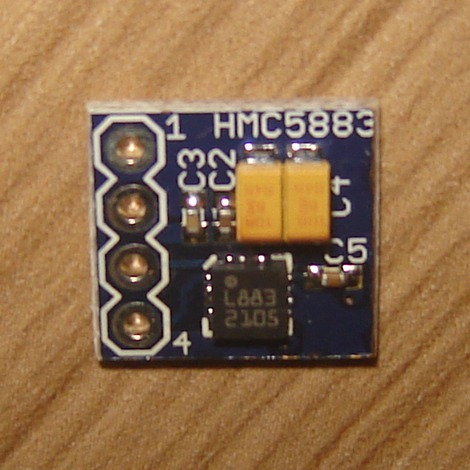
\includegraphics[width=0.45\textwidth]{img/sensor_front.jpg}
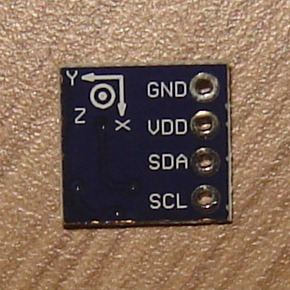
\includegraphics[width=0.45\textwidth]{img/sensor_back.jpg}
\caption{Fotos da PCB contendo o sensor}
\label{fig:sensor_photos}
\end{figure}


\chapter{Descrição do \textit{hardware}}
\label{cap:hardware}

O núcleo do circuito é o microcontrolador ATmega8, o qual é responsável por
ler os dados do sensor, fazer cálculos para converter os valores lidos, e
enviar as coordenadas via \ac{USB}.

Um cristal de \SI{12}{\mega\hertz}, ligado aos pinos 9 e 10, define o
\textit{clock} do microcontrolador. O \textit{driver} usado para a
implementação do protocolo \ac{USB}, descrito na seção \ref{sec:vusb},
permite o uso de cristais de \SIlist[list-final-separator={ ou }]{12; 15;
16; 20}{\mega\hertz}. A escolha pelo cristal de \SI{12}{\mega\hertz} foi
arbitrária.

O pino 1 (\textoverline{RESET}) possui um resistor de \textit{pull-up}
(ligado ao \VCC) e um botão ligado ao \GND. Quando o botão é pressionado, o
nível lógico do pino cai para zero e o microcontrolador é reiniciado. Este
botão de \textit{reset} se mostrou bastante útil durante o desenvolvimento,
mas não é necessário para o funcionamento deste projeto.

Há 3 \acp{LED} ligados aos pinos 11, 12 e 13 (PORTD5, PORTD6, PORTD7),
montados de modo a acender quando o valor lógico 1 é escrito. Foram usados
para fins de depuração, mas não são essenciais para o funcionamento deste
projeto.

Há 3 botões ligados aos pinos 23, 24 e 25 (PORTC0, PORTC1, PORTC2), e ainda
uma chave ligada ao pino 26 (PORTC3). Quando pressionados, o nível lógico de
cada pino cai para zero. Cada pino possui internamente um resistor de
\textit{pull-up}, o qual foi habilitado pelo programa, dispensando o uso de
resistores externos.

Os pinos 17, 18 e 19 (MOSI, MISO, SCK), juntamente com o pino 1
(\textoverline{RESET}) são usados para \ac{ISP}. Por simplicidade e por
falta de necessidade, decidiu-se não usá-los para nenhuma outra função.

Por fim, os pinos 2 e 4 (PD0 e PD2) estão ligados às vias USB~D- e USB~D+, e
serão detalhados na seção \ref{sec:hardware_usb}; e os pinos 27 e 28 (SDA e
SCL) estão ligados ao sensor através de um barramento \ac{I2C}, e serão
detalhados na seção \ref{sub:hardware_sensor_i2c}.

\begin{figure}[h]
\centering
\includegraphics[width=1.0\textwidth]{img/circuito-USBasp.pdf}
\caption{Diagrama completo do circuito}
\label{fig:circuito_completo}
\end{figure}

% TODO: Atualizar o diagrama do circuito!


\section{Interface USB}
\label{sec:hardware_usb}

Um porta \ac{USB} fornece \SI{5}{\volt} na via \VBUS, porém a especificação
limita as vias de dados D+ e D- ao intervalo de \SIrange{2.8}{3.6}{\volt}.
\cite[p.~178,~179]{usb20}

Uma solução seria usar um microcontrolador que possa funcionar a tensões
mais baixas e colocar um circuito para reduzir a alimentação para dentro do
intervalo desejado. Modelos mais recentes da linha AVR permitem o uso dessa
solução. \cite[p.~322]{ATmega_newer_datasheets} No entanto, o
microcontrolador ATmega8 usado neste projeto não trabalha com tensões
inferiores a \SI{4.5}{\volt}. \cite{ATmega8}

Uma outra solução é manter o microcontrolador alimentado com \SI{5}{\volt} e
adicionar um circuito para reduzir a saída dos pinos do AVR para a tensão
desejada. Esta foi a solução empregada neste projeto.

O circuito usado para reduzir a tensão nas linhas de dados segue o mesmo
esquema usado no projeto USBasp \cite{USBasp}, também disponível no arquivo
\texttt{circuits/with-zener.png} do \textit{driver} \VUSB \cite{vusbdrv}. É
composto de um diodo Zener de \SI{3.6}{\volt} ligando a linha de dados ao
\GND, e um resistor de \SI{68}{\ohm} entre o microcontrolador e o diodo
Zener.

Quando o microcontrolador escreve o nível lógico 1, seu pino sobe para
\SI{5}{\volt}. Como essa tensão é maior que a tensão de ruptura do Zener,
este começa a conduzir, limitando a tensão da linha de dados. A diferença de
$\num{5} - \num{3.6} = \SI{1.4}{\volt}$ fica no resistor, resultando numa
corrente de $\SI{1.4}{\volt} / \SI{68}{\ohm} = \SI{20.6}{\milli\ampere}$,
que é abaixo do limite de \SI{40}{\milli\ampere} para cada pino do
microcontrolador. \cite[p.~235]{ATmega8}

Além disso, conforme mencionado na seção \ref{sec:usb}, é preciso adicionar
um resistor de \textit{pull-up} à linha D-, indicando que este dispositivo
é \textit{low speed}. A especificação do USB 2.0 define que esse resistor
deve ter \SI{1.5}{\kilo\ohm}. \cite[p.~141,~180]{usb20} O projeto USBasp, no
entanto, usa um resistor de \SI{2.2}{\kilo\ohm} \cite{USBasp}, que, mesmo
fora da especificação, também funcionou.

Por fim, para o funcionamento correto do \textit{driver} \VUSB, é necessário
ligar a linha USB~D+ ao pino INT0 do microcontrolador. Além disso, é preciso
que as duas vias de dados estejam ligadas a pinos que pertençam à mesma
porta do microcontrolador. \cite[usbconfig-prototype.h]{vusbdrv} Portanto, a
linha D+ foi ligada ao pino 4 (PD2/INT0), e a linha D- foi ligada ao pino 2
(PD0).


\section{Interface com o sensor}
\label{sec:hardware_sensor}

\subsection{Alimentação}
\label{sub:hardware_sensor_alimentacao}

O sensor HMC5883L trabalha com alimentação de \SIrange{2.16}{3.6}{\volt}.
\cite[p.~2]{HMC5883L} Como a \ac{USB} fornece \SI{5}{\volt}, é necessário
adicionar um circuito para reduzir a tensão até um nível adequado.

A solução aqui empregada utiliza um diodo Zener de \SI{3.3}{\volt} e um
resistor de \SI{470}{\ohm}. \cite{3vtipsandtricks} É bastante similar àquela
descrita na seção \ref{sec:hardware_usb}, mudando apenas os valores dos
componentes.

O diodo Zener e o resistor estão ligados em série entre \VCC e \GND,
drenando constantemente uma corrente de $ (\SI{5}{\volt} - \SI{3.3}{\volt})
/ \SI{470}{\ohm} = \SI{3.6}{\milli\ampere} $ e mantendo a tensão de
\SI{3.3}{\volt} em relação ao \GND entre esses dois componentes.

Considerando que o sensor drena apenas \SI{0.1}{\milli\ampere} quando em
uso \cite[p.~2]{HMC5883L}, a queda de tensão na alimentação quando em carga
é desprezível, e portanto essa solução é bastante adequada para este
propósito.

\subsection{Barramento I²C}
\label{sub:hardware_sensor_i2c}

% TODO: level-shifting do I²C
TODO: Descrever o level shifting para I²C. \cite{AN97055} \cite{AN10441}
Falar também do resistor de \textit{pull-up}.


\chapter{Descrição do \textit{software}}
\label{cap:software}

O \textit{firmware} deste projeto foi desenvolvido em ambiente Linux x86\_64,
utilizando o compilador AVR-GCC versão 4.5.3, a biblioteca AVR-Libc versão
1.7.0 e as ferramentas do projeto Binutils versão 2.21.1. O código-fonte foi
escrito na linguagem C e é facilmente portável para outros
microcontroladores da família AVR. Para gravação do \textit{firmware} no
microcontrolador, foi usado o programa AVRDUDE.

Todo o ambiente de desenvolvimento usado (AVR-GCC, Binutils, AVR-Libc,
AVRDUDE) é composto por \textit{software} livre e é está disponível para os
principais sistemas operacionais (FreeBSD, Linux, Mac OS X e Windows).
\cite{avrlibcoverview}

O \textit{firmware} deste projeto pode ser compilado em qualquer sistema
operacional que tenha as ferramentas citadas, mesmo em outras versões,
embora alguns ajustes no Makefile possam ser necessários.


\section{Boot loader}
\label{sec:bootloader}

Durante o início do projeto, o ciclo de desenvolvimento podia ser resumido
nestas etapas:

\begin{enumerate}
\item Compilar o código-fonte.
\item Desconectar a \textit{protoboard} da \ac{USB}.
\item Conectar o gravador de AVR na \ac{USB}.
\item Gravar a nova versão do \textit{firmware}.
\item Desconectar o gravador de AVR.
\item Reconectar a \textit{protoboard} na \ac{USB}.
\end{enumerate}

Rapidamente esse processo se mostrou bastante demorado e ineficiente,
atrasando os testes e a depuração do código recém-escrito, e portanto
atrasando o desenvolvimento. Além disso, também causava um desgaste mecânico
desnecessário na porta \ac{USB}. Embora esse desgaste seja desprezível a
curto prazo, poderia se tornar um problema real para projetos de longo
prazo.

Visando agilizar e simplificar o ciclo de desenvolvimento, foi gravado um
\textit{boot loader} na região de \textit{boot} do microcontrolador.

Foi usado o USBaspLoader \cite{USBaspLoader} como \textit{boot loader}. Ele
foi escolhido por ser \textit{open source} e por também usar o
\textit{driver} \VUSB, o qual será descrito em mais detalhes na seção
\ref{sec:vusb}.

Um \textit{boot loader} é gravado nos endereços mais altos da memória
\textit{Flash}. O microcontrolador ATmega8 tem suporte a \textit{boot
loaders} de tamanhos \numlist{256;512;1024;2048} bytes.
\cite[p.~213]{ATmega8} Após compilado, o USBaspLoader possui \num{2028}
bytes, e portanto ocupa os \num{2048} bytes superiores da memória
\textit{Flash}.

Logo após um \textit{reset}, o ATmega8 normalmente começaria a execução do
programa a partir do endereço mais baixo da memória. No entanto, quando se
ativa o \textit{boot loader} (através dos \textit{fuse bits} do
microcontrolador \cite[p.~216]{ATmega8}), a execução começa no endereço da
região de \textit{boot}.

Portanto, ao iniciar o microcontrolador, o USBaspLoader é executado antes do
\textit{firmware} principal. Se uma determinada condição (configurável) for
verdadeira, então o USBaspLoader assume o controle e se identifica como um
gravador USBasp\footnote{
	USBasp é um gravador de AVR com conexão USB que é implementado usando um
	microcontrolador ATmega8 ou similar. \cite{USBasp}
}.
Caso essa condição seja falsa (antes ou durante a execução do USBaspLoader),
então o \textit{firmware} principal é executado.

Com o uso deste \textit{boot loader}, o ciclo de desenvolvimento foi
reduzido para:

\begin{enumerate}
\item Compilar o código-fonte.
\item Deixar ligada a chave conectada ao pino 26 (PORTC3) do
microcontrolador.
\item Apertar o botão de \textit{reset}.
\item Gravar a nova versão do \textit{firmware}.
\end{enumerate}

Após receber uma nova versão do \textit{firmware} principal, o USBaspLoader
automaticamente inicia a execução desse \textit{firmware} recém-gravado.

Com o uso de um \textit{boot loader}, o ciclo de desenvolvimento tornou-se
notavelmente mais rápido e dinâmico. Testar mudanças no \textit{firmware}
passou a ser fácil, e os testes se tornaram mais frequentes.

Como desvantagem, o espaço disponível na memória \textit{Flash} do
microcontrolador foi reduzido de \num{8192} para \num{6144} bytes.


\section{Comunicação I²C/TWI}
\label{sec:twi}

O microcontrolador ATmega8 possui um \textit{hardware} dedicado para
comunicação \ac{I2C} (chamada de \ac{TWI}, conforme citado na seção
\ref{sec:atmega8}). No entanto, seu uso é relativamente burocrático, tendo
que implementar uma máquina de estados para gerenciar os registradores do
módulo de \ac{TWI} e a transmissão de dados. \cite[p.~168]{ATmega8} O
exemplo de código disponível na página 170 do \textit{datasheet} do ATmega8
utiliza a técnica de \textit{busy-wait} e não é adequado para o firmware
deste projeto.\footnote{
	De maneira geral, a técnica de \textit{busy-wait} (espera ocupada) deve
	ser evitada porque bloqueia a execução do restante do código por tempo
	indeterminado. Isso causaria, portanto, um \textit{watchdog reset}. Além
	disso, a espera ocupada não garantiria que a função \texttt{usbPoll()}
	fosse chamada em intervalos menores que \SI{50}{\milli\second}, conforme
	descrito na seção \ref{sub:vusb_config}.}

Reconhecendo a dificuldade de usar esse módulo de maneira eficiente, a
própria \textit{Atmel} publicou um documento e o código-fonte de um
\textit{driver}\footnote{
	Neste contexto, ``\textit{driver}'' significa um pedaço de
	\textit{software} dentro do \textit{firmware} que controla um módulo de
	hardware do microcontrolador. Não confundir com \textit{drivers} do
	sistema operacional.}
que utiliza o módulo \ac{TWI} de maneira mais eficiente. \cite{AVR315}

Para este projeto, foi usado o \textit{driver} disponível na
\textit{application note} ``AVR315: Using the TWI module as I²C master''.
Seu funcionamento é baseado em interrupções, e portanto pode realizar a
transmissão de vários bytes de maneira assíncrona (não-bloqueante), uma
característica altamente desejável. A rotina de tratamento da interrupção
basicamente implementa uma máquina de estados. \cite[p.~13]{AVR315}

O \textit{driver} possui um \textit{buffer} interno para armazenar os dados
a serem enviados ou os dados sendo recebidos. O tamanho desse
\textit{buffer} é configurável em tempo de compilação, através da linha:

\begin{ccode}[numbers=none]
#define TWI_BUFFER_SIZE     7
\end{ccode}

O código-fonte estava originalmente escrito para o compilador IAR. Adaptá-lo
para o compilador GCC foi uma tarefa bastante simples, bastando apenas
trocar os cabeçalhos e trocar a sintaxe da declaração da rotina de
interrupção. \cite{avrlibcporting}

\begin{ccode}[numbers=none, multicols=2, float=h]
// IAR:
#include "ioavr.h"
#include "inavr.h"
// GCC:
#include <avr/io.h>
#include <avr/interrupt.h>
\end{ccode}

\begin{ccode}[numbers=none, multicols=2, float=h]
// IAR syntax:
#pragma vector=TWI_vect
__interrupt void TWI_ISR(void)
{
  ...
}
// GCC syntax:
ISR(TWI_vect)
{
  ...
}

\end{ccode}


\section{Comunicação com o sensor}
\label{sec:software_sensor}

O sensor HMC5883L possui 13 registradores de 8 bits que podem ser acessados
pela comunicação serial, e ainda mais um registrador interno chamado de
\textit{address pointer}, o qual aponta para algum dos outros registradores
e cujo valor não pode ser lido. \cite[p.~11]{HMC5883L}

Quando o \textit{master} inicia uma escrita, o primeiro byte recebido pelo
sensor é considerado o endereço de um registrador, e esse endereço é salvo
no \textit{address pointer}. Caso um segundo byte seja recebido, esse valor
é salvo no registrador apontado pelo \textit{address pointer}.

Assim, para escrever num dos registradores de configuração do sensor, o
\textit{firmware} do microcontrolador prepara um vetor de 3 bytes: o
endereço do sensor (juntamente com o bit que define uma operação de
escrita), o número do registrador de configuração que será modificado, e o
valor a ser escrito no registrador. Esse vetor é repassado ao
\textit{driver} de \ac{TWI} (descrito na seção \ref{sec:twi}), o qual copia
esses bytes para um \textit{buffer} interno e inicia a comunicação
assincronamente.

Quando o \textit{master} inicia uma leitura, o sensor envia um byte com o
valor contido no registrador apontado pelo \textit{address pointer} e
incrementa o \textit{address pointer} para apontar para o próximo
registrador. Caso outro byte seja requisitado (ainda na mesma transmissão,
ou em outra transmissão), o processo se repete, enviado o valor contido no
registrador apontado pelo \textit{address pointer} e incrementando-o. Desta
forma, é possível ler o conteúdo de vários registradores adjacentes de
maneira bem eficiente, com \textit{overhead} de comunicação mínimo.

No entanto, a implementação do sensor não é perfeita, e em certos casos ao
auto-incremento do \textit{address pointer} não funciona como esperado. Por
exemplo, uma tentativa de ler todos os registradores (usando o
auto-incremento para iterar automaticamente por todos eles) retorna valores
diferentes (e inválidos) daqueles retornados por leituras individuais. De
maneira geral, o auto-incremento funciona corretamente apenas para leitura
dos 6 registradores de dados e para a leitura dos 3 registradores de
identificação do sensor.

Para ler os valores X, Y, Z do sensor, o microcontrolador começa realizando
uma escrita no sensor, enviando o valor \texttt{0x03} como endereço do
registrador. A seguir, realiza uma leitura de 6 bytes consecutivos. Por fim,
esses 6 bytes lidos são convertidos numa \texttt{struct} de 3 variáveis
inteiras de 16 bits.

\subsection{Configuração do sensor}
\label{sub:software_sensor_config}

Durante a inicialização do \textit{firmware} do microcontrolador, os
registradores de configuração do sensor são escritos.

O sensor foi configurado para atualizar os registradores de dados 75 vezes
por segundo, sendo que cada valor é a média de 8 amostras. O ganho do sensor
foi configurado para ±\SI{1.3}{\gauss}\footnote{
	O símbolo \si{\gauss} corresponde à unidade de medida de campo magnético
	``gauss'' \cite[p.~128]{SI}. O \textit{datasheet} do sensor, no entanto,
	utiliza Ga como símbolo para essa unidade.
}, o que corresponde a 1090 bits por gauss, ou \SI{0.92}{\milli\gauss} por
bit. Este ganho foi escolhido por ser permitir a maior precisão possível das
medidas sem causar \textit{overflow} no sensor.

O sensor foi configurado para o modo de medição contínua, \ie, está
continuamente medindo o campo magnético e atualizando os registradores de
dados (75 vezes por segundo), mesmo que o microcontrolador não faça a
leitura dessas medidas. Essa abordagem foi escolhida por simplificar a
implementação.

Por limitação do sensor, esse modo permite obter medições a uma taxa máxima
de \SI{75}{\hertz}. Apesar disso, o sensor permite medições a até
\SI{160}{\hertz} se for configurado para realizar medições individuais e o
pino DRDY for monitorado. \cite[p.~12]{HMC5883L} Este pino normalmente fica
no nível lógico 1, porém cai para 0 por \SI{250}{\micro\second} assim que
uma nova medida é colocada nos registradores de dados. \cite[p.~3]{HMC5883L}
Portanto, seria possível ligar esse pino DRDY a algum dos pinos de
interrupção do microcontrolador e escrever uma rotina que leia os dados e
inicie a próxima medição.

Todavia, a \ac{PCB} usada neste projeto (figura \ref{fig:sensor_photos}) não
possui um contato para o pino DRDY, e portanto não foi possível se
aproveitar dessa técnica.


\section{\textit{Driver} \VUSB}
\label{sec:vusb}

O \textit{driver} \VUSB foi desenvolvido pela \textit{Objective Development
Software GmbH.} e é uma implementação em \textit{software} do protocolo
\ac{USB}, funcionando em diversos microcontroladores da família AVR que não
possuem um controlador \ac{USB} embutido. \cite{VUSBdriver}

Por ser implementado em \textit{software}, o tempo de execução das rotinas
do \textit{driver} é crucial, e essas rotinas foram implementadas (pelos
autores do \textit{driver}) em \textit{assembly} para \textit{clocks} de
\SIlist[list-final-separator={ ou }]{12; 15; 16; 20}{\mega\hertz} usando
cristal, ou \SIlist[list-final-separator={ ou }]{12.8; 16.5}{\mega\hertz}
usando o oscilador interno do microcontrolador. Não é possível usar o
\textit{driver} com frequências diferentes destas. \cite{VUSBdriver}

Apesar das rotinas internas estarem escritas em \textit{assembly}, o
\textit{driver} disponibiliza uma \ac{API} bastante simples em linguagem C.

O \textit{driver} implementa um dispositivo \ac{USB} 1.1 \textit{low speed},
mas possui algumas limitações. Uma delas é assumir que não há erros durante
a comunicação, pois não há tempo de CPU suficiente para implementar checagem
de erros via \textit{software}. Além disso, as características elétricas dos
pinos não atendem estritamente a especificação \ac{USB}. \cite{VUSBdriver}

A especificação \ac{USB} também define que os dispositivos devem implementar
um modo \textit{suspend}, no qual não devem consumir mais que
\SI{500}{\micro\ampere}. \cite[cap.~2]{usbinanutshell} O \textit{driver} não
implementa esse modo, mas explica em linhas gerais como seria possível
implementá-lo. \cite[usbdrv.h]{VUSBdriver} Para este projeto, não foi
implementado o suporte ao modo \textit{suspend}, pois não é uma tarefa
trivial e está fora do escopo deste trabalho.

Considerando as limitações citadas nos parágrafos anteriores, o dispositivo
fruto deste projeto não é totalmente conformante com a especificação
\ac{USB}. Por outro lado, essas limitações não são críticas, e o dispositivo
funciona corretamente.


\subsection{Configuração do \textit{driver} \VUSB}
\label{sub:vusb_config}

Toda a configuração do \textit{driver} \VUSB é feita no arquivo
\texttt{usbconfig.h}. Como a maior parte da configuração é compartilhada com
o \textit{boot loader}, foi criado um arquivo \texttt{hardwareconfig.h} que
contém as configurações compartilhadas entre o \textit{firmware} principal e
o \textit{boot loader} (tais como em quais pinos estão ligadas as linhas D-
e D+), enquanto as configurações específicas foram mantidas no arquivo
\texttt{usbconfig.h}.

Para o \textit{firmware} principal, foi habilitado um \textit{interrupt-in
endpoint} com intervalo \textit{polling} de \SI{10}{\milli\second} (o menor
valor possível para dispositivos \textit{low speed})

TODO FROM HERE (e revisar o parágrafo anterior)



%Falar sobre o consumo de 100mA.
%Falar sobre os tipos de endpoints.


\section{Teclado USB}
\label{sec:keyboard}

Falar aqui sobre a implementação de um teclado.


\section{Menu de configuração}
\label{sec:menu}

Talvez falar sobre o teclado aqui dentro, não sei.

\section{Transformação de coordenadas}
\label{sec:coordenadas}

Falar sobre: ferramentas auxiliares, teoria, resultados.

Falar sobre calibração dos cantos.

Falar sobre calibração do zero (ou deixar para falar isso depois).

\section{Mouse USB}
\label{sec:mouse}

Falar sobre a implementação do mouse (que na verdade é absolute pointing
device).

Talvez aqui, talvez numa outra (sub)seção, falar sobre o fluxo da main().

\section{Outros problemas}
\label{sec:outros_problemas}


Em algum lugar (seção "outros problemas encontrados", por exemplo), citar o
problema ao realizar muitas leituras muito rapidamente, cuja solução foi
realizar leituras num timer.


\subsection{Debouncing dos botões}
\label{sec:debouncing}

\subsection{Tamanho do firmware}
\label{sec:firmware_size}

Dentre outras coisas, falar sobre as flags de compilação, que são
específicas para a versão 4.5 do GCC.

\subsection{Gravar configurações na EEPROM}
\label{sec:eeprom}

Falar sobre gravar na EEPROM de maneira não bloqueante.

\chapter{Conclusões}
\label{cap:conclusoes}

Resultados alcançados. O que deu certo. O que não deu certo.

\section{Trabalhos futuros}
\label{sec:trabalhos_futuros}

Listar o que pode ser feito a partir deste projeto.


TODO: falar sobre o pino DRDY

\begin{figure}[h]
\centering
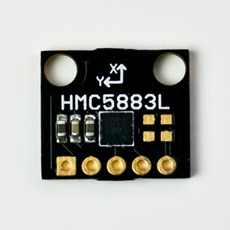
\includegraphics[width=0.45\textwidth]{img/sensor_other_pcb_top.jpg}
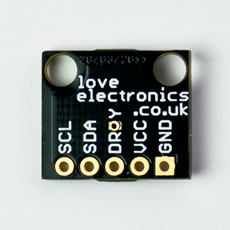
\includegraphics[width=0.45\textwidth]{img/sensor_other_pcb_bottom.jpg}
\caption{Fotos de uma PCB com 5 contatos disponíveis}
\label{fig:loveelectronics_photos}
\end{figure}

% TODO: falar sobre o pino DRDY (talvez falar isso só nas conclusões, ou na
% seção onde se configura o sensor



%%fakesection  Bibliografia

\bibliographystyle{abnt-num}
\bibliography{mouse_magnetometro_monografia}

% How to add \url{} to "url=" entries from Pybliographic:
% :%s/\(url\s*=\s*{\)\([^\\].*[^}]\)\(},\?\)/\1\\url{\2}\3/


%%fakesection  Apendice
\apendice

% Aproximadamente 84 páginas.
% Mais páginas, se inserir um pagebreak/chapter antes de cada arquivo.
%\lstinputlisting[language=C]{../firmware/avr315/TWI_Master.h}
%\lstinputlisting[language=C]{../firmware/avr315/TWI_Master.c}
%\lstinputlisting[language=C]{../firmware/buttons.h}
%\lstinputlisting[language=C]{../firmware/buttons.c}
%\lstinputlisting[language=C]{../firmware/common.h}
%\lstinputlisting[language=C]{../firmware/int_eeprom.h}
%\lstinputlisting[language=C]{../firmware/int_eeprom.c}
%\lstinputlisting[language=C]{../firmware/keyemu.h}
%\lstinputlisting[language=C]{../firmware/keyemu.c}
%\lstinputlisting[language=C]{../firmware/main.c}
%\lstinputlisting[language=C]{../firmware/menu.h}
%\lstinputlisting[language=C]{../firmware/menu.c}
%\lstinputlisting[language=C]{../firmware/mouseemu.h}
%\lstinputlisting[language=C]{../firmware/mouseemu.c}
%\lstinputlisting[language=C]{../firmware/sensor.h}
%\lstinputlisting[language=C]{../firmware/sensor.c}
%\lstinputlisting[language=C]{../firmware/hardwareconfig.h}
%\lstinputlisting[language=C]{../firmware/usbconfig.h}


%%fakesection  Anexo
\anexo


\chapter{ATmega8 datasheet}
\label{anx:atmega8_datasheet}

Páginas 1-6, 9-10, 17-19, 157-160, 168-170, 213, 216-217, 235-236, 238-239, 280-284. \cite{ATmega8}

\includepdf[pages={1-6, 9-10, 17-19, 157-160, 168-170, 213, 216-217, 235-236, 238-239, 280-284}]{/home/denilson/avr/PDFs/doc2486.pdf}


\chapter{HMC5883L datasheet}
\label{anx:hmc5883l_datasheet}

Todas as páginas. \cite{HMC5883L}

\includepdf[pages={-}]{../../hmc5883/HMC5883L.pdf}


\chapter{3V Tips 'n Tricks}
\label{anx:3vtipsandtricks_pdf}

Páginas 1, 4. \cite{3vtipsandtricks}

\includepdf[pages={1, 4}]{../../level-shifting/en026368.pdf}


\chapter{AVR315: Using the TWI module as I²C master}
\label{anx:avr315_pdf}

Todas as páginas. \cite{AVR315}

\includepdf[pages=-]{/home/denilson/avr/PDFs/doc2564.pdf}


\end{document}

% vim:filetype=tex ts=4 sw=4 noet tw=76
